\documentclass[tikz,crop]{standalone}

\usepackage{tikz,pgfplots}
\usepackage{physics}

\usetikzlibrary{decorations.shapes}
\usetikzlibrary{arrows.meta,calc,decorations.markings,math,arrows.meta}
\usetikzlibrary{%
    decorations.pathreplacing,%
    decorations.pathmorphing%
}


%------------   Todo está en 2D porque no entiendo 3D   :c    ------------%


\begin{document}

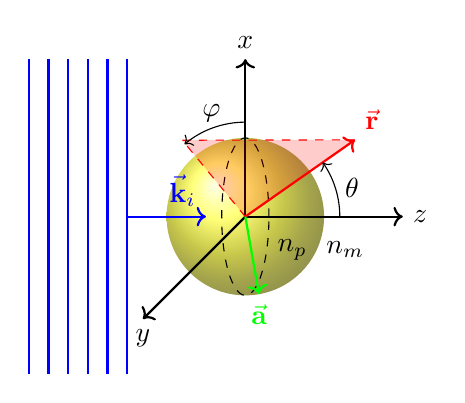
\begin{tikzpicture}[scale=1]

\coordinate (O) at (0,0);

%------------------------------------------------------- Particle
\shade[ball color=yellow, opacity = .7] (O) circle (1); 
\draw[dashed] (O) ellipse (.3 and 1);

%------------------------------------------------------- Coordinate system axes
\draw[thick,->] (O) -- (-1.3,-1.3) node[anchor=north ]{$y$};
\draw[thick,->] (O) -- (2,0) node[anchor= west]{$z$};
\draw[thick,->] (O) -- (0,2) node[anchor=south]{$x$};


%------------------------------------------------------- Vector \va{r}
\draw[thick,red,->] (O) -- (35:1.7) node[anchor=south west]{$\va{r}$}; 
\draw[-, dashed,red] (O) -- (-.8,.97);		%xy proyection
\draw[-,dashed,red] (-.8,.97) -- (35:1.7) ;	%normal proyection
\fill[red,opacity=.2] (O)-- (-.8,.97)--(35:1.7)--(O);  %Shade
	
	
%------------------------------------------------------- polar variables	
\path (O)++(35/2:1.2)node[anchor=west]{$\theta$};    
\draw[->](0:1.2)arc(0:35:1.2);

\path (O)++(100:1.1)node[anchor=south east]{$\varphi$};    
\draw[->](90:1.2)arc(90:130:1.2);
	

%------------------------------------------------------- Particule radius & n	
\draw[thick,green,->] (O) -- (-80:1) node[anchor=north]{$\va{a}$};  

\path (O)++(-25:1) node[anchor=east]{$n_p$};
\path (O)++(-25:1) node[anchor=west]{$n_m$};


%------------------------------------------------------- Plane wave

\foreach \i in {-5,...,-1,0}{
	\draw[thick,blue] (\i*.25-1.5,-2)--(\i*.25-1.5,2);}
\draw[->,thick,blue] (-1.5,0)--(-1.5+1,0) node[anchor=south east]{$\va{k}_i$};

	
\end{tikzpicture}
\end{document}